%%%%%%%%%%%%%%%%%%%%%%%%%%%%%%%%%%%%%%%%%%%%%%%%%%%%%%%%%%%%%%%%%%%%%%%%%%%%%%%%%%
\begin{frame}[fragile]\frametitle{}
\begin{center}
{\Large Introduction to Ludwig}

{\tiny (Ref: Efficiently Build Custom LLMs on Your Data - https://www.youtube.com/watch?v=NAyKpcOdHLE - Piero Molino,  Arnav Garg)}

\end{center}
\end{frame}


%%%%%%%%%%%%%%%%%%%%%%%%%%%%%%%%%%%%%%%%%%%%%%%%%%%%%%%%%%%
\begin{frame}[fragile]\frametitle{Current State of ML Projects}


		\begin{center}
		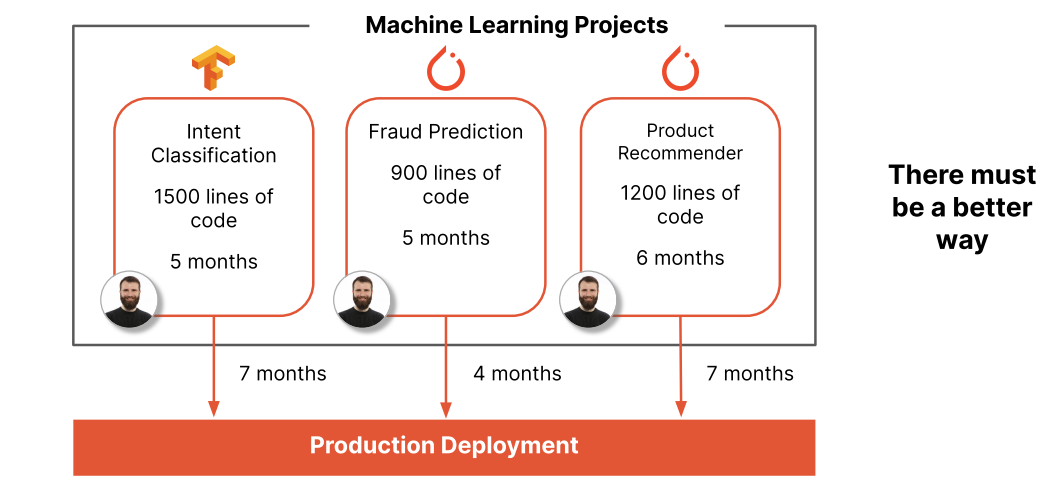
\includegraphics[width=\linewidth,keepaspectratio]{ludwig1}
		\end{center}

Lot of time needed, many pieces are boiler-plate.
\end{frame}


%%%%%%%%%%%%%%%%%%%%%%%%%%%%%%%%%%%%%%%%%%%%%%%%%%%%%%%%%%%
\begin{frame}[fragile]\frametitle{Solution by LUDWIG}


		\begin{center}
		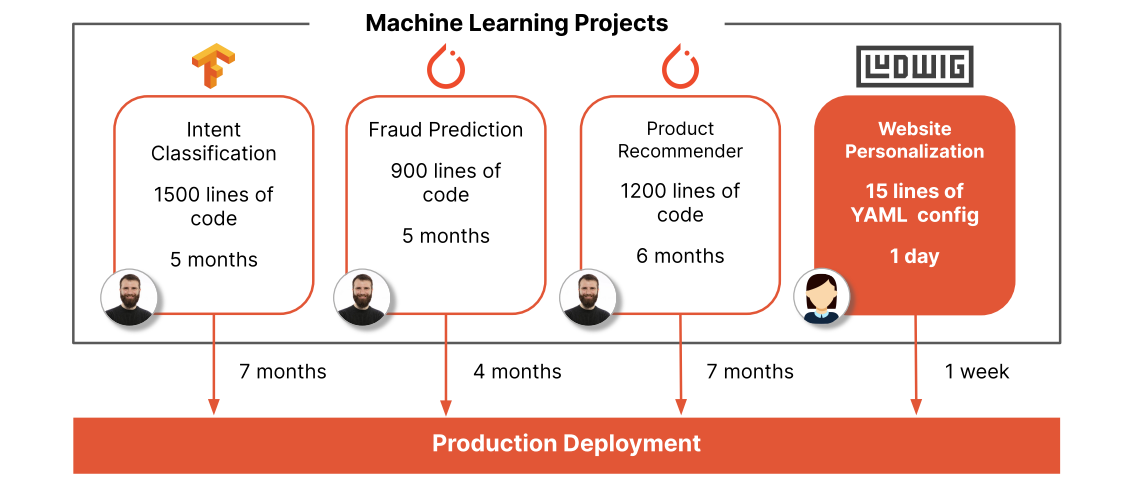
\includegraphics[width=\linewidth,keepaspectratio]{ludwig2}
		\end{center}

\end{frame}

%%%%%%%%%%%%%%%%%%%%%%%%%%%%%%%%%%%%%%%%%%%%%%%%%%%%%%%%%%%
\begin{frame}[fragile]\frametitle{Flexibility Levels}


		\begin{center}
		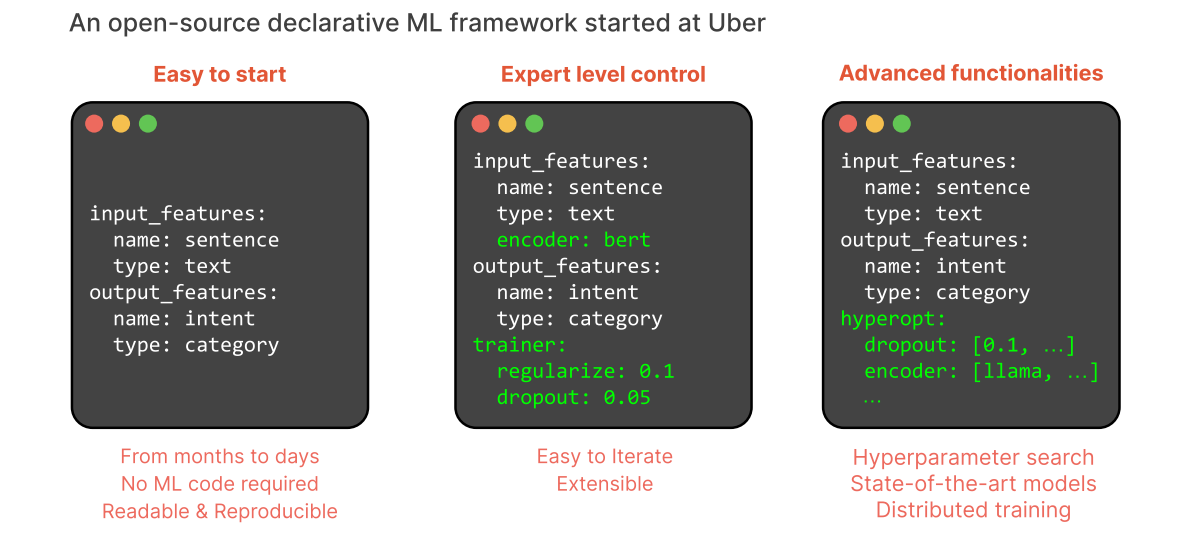
\includegraphics[width=\linewidth,keepaspectratio]{ludwig3}
		\end{center}

Just specify what you want (declarative) and not how to get it done.
Iterating on different customization is easy. Just change the config and run!!

\end{frame}


%%%%%%%%%%%%%%%%%%%%%%%%%%%%%%%%%%%%%%%%%%%%%%%%%%%%%%%%%%%%%%%%%%%%%%%%%%%%%%%%%%
\begin{frame}[fragile]\frametitle{Introduction}
    \begin{itemize}
        \item Large Language Models (LLMs) have revolutionized NLP tasks.
        \item Fine-tuning LLMs for specific tasks is crucial.
        \item Ludwig framework from Pedibase offers efficient fine-tuning.
    \end{itemize}
\end{frame}


%%%%%%%%%%%%%%%%%%%%%%%%%%%%%%%%%%%%%%%%%%%%%%%%%%%%%%%%%%%%%%%%%%%%%%%%%%%%%%%%%%
\begin{frame}[fragile]\frametitle{Large Language Modeling Fine-Tuning using Ludwig}
\begin{itemize}
    \item Ludwig: Open-source AI toolbox by Uber
    \item Supports fine-tuning of pre-trained language models
    % \item Supports popular models like BERT, RoBERTa, GPT-2
    \item Provides easy-to-use data preprocessing and model training
    \item Supports multi-task learning and transfer learning
    \item Flexible data input formats (CSV, JSON, pandas DataFrame)
    \item Automatic metric computation and visualizations
    \item Distributed training support %(Horovod, Ray)
    \item Serialization and deployment of trained models
    \item Active development and community support
\end{itemize}
\end{frame}


%%%%%%%%%%%%%%%%%%%%%%%%%%%%%%%%%%%%%%%%%%%%%%%%%%%%%%%%%%%%%%%%%%%%%%%%%%%%%%%%%%
\begin{frame}[fragile]\frametitle{Setup}
    \begin{itemize}
        \item Install Ludwig framework: \lstinline{pip install ludwig}.
        \item Prepare data in required format.
        \item Define model architecture and parameters.
    \end{itemize}
\end{frame}

%%%%%%%%%%%%%%%%%%%%%%%%%%%%%%%%%%%%%%%%%%%%%%%%%%%%%%%%%%%%%%%%%%%%%%%%%%%%%%%%%%
\begin{frame}[fragile]\frametitle{Fine-tuning Process}
    \begin{itemize}
        \item Load pre-trained LLM using Ludwig.
        \item Specify task-specific data for fine-tuning.
        \item Train the model with Ludwig's \lstinline{train} command.
    \end{itemize}
\end{frame}

%%%%%%%%%%%%%%%%%%%%%%%%%%%%%%%%%%%%%%%%%%%%%%%%%%%%%%%%%%%%%%%%%%%%%%%%%%%%%%%%%%
\begin{frame}[fragile]\frametitle{Task-Specific Tuning}
    \begin{itemize}
        \item Adapt pre-trained LLM to specific tasks (e.g., text generation, classification).
        \item Configure task-specific parameters (e.g., learning rate, batch size).
        \item Fine-tune on task-specific data.
    \end{itemize}
\end{frame}

%%%%%%%%%%%%%%%%%%%%%%%%%%%%%%%%%%%%%%%%%%%%%%%%%%%%%%%%%%%%%%%%%%%%%%%%%%%%%%%%%%
\begin{frame}[fragile]\frametitle{Evaluation}
    \begin{itemize}
        \item Assess fine-tuned model performance using evaluation metrics.
        \item Validate against task-specific benchmarks.
        \item Iterate fine-tuning process if necessary.
    \end{itemize}
\end{frame}

%%%%%%%%%%%%%%%%%%%%%%%%%%%%%%%%%%%%%%%%%%%%%%%%%%%%%%%%%%%%%%%%%%%%%%%%%%%%%%%%%%
\begin{frame}[fragile]\frametitle{Hyperparameter Optimization}
    \begin{itemize}
        \item Tune hyperparameters for optimal performance.
        \item Ludwig supports hyperparameter search.
        \item Utilize techniques like grid search or random search.
    \end{itemize}
\end{frame}

%%%%%%%%%%%%%%%%%%%%%%%%%%%%%%%%%%%%%%%%%%%%%%%%%%%%%%%%%%%%%%%%%%%%%%%%%%%%%%%%%%
\begin{frame}[fragile]\frametitle{Deployment}
    \begin{itemize}
        \item Deploy fine-tuned model for inference.
        \item Integrate with existing applications or services.
        \item Monitor model performance in production.
    \end{itemize}
\end{frame}


%%%%%%%%%%%%%%%%%%%%%%%%%%%%%%%%%%%%%%%%%%%%%%%%%%%%%%%%%%%
\begin{frame}[fragile]\frametitle{Ludwig Architecture}

Many NLP tasks can be abstracted to Sequence To Sequence model.

		\begin{center}
		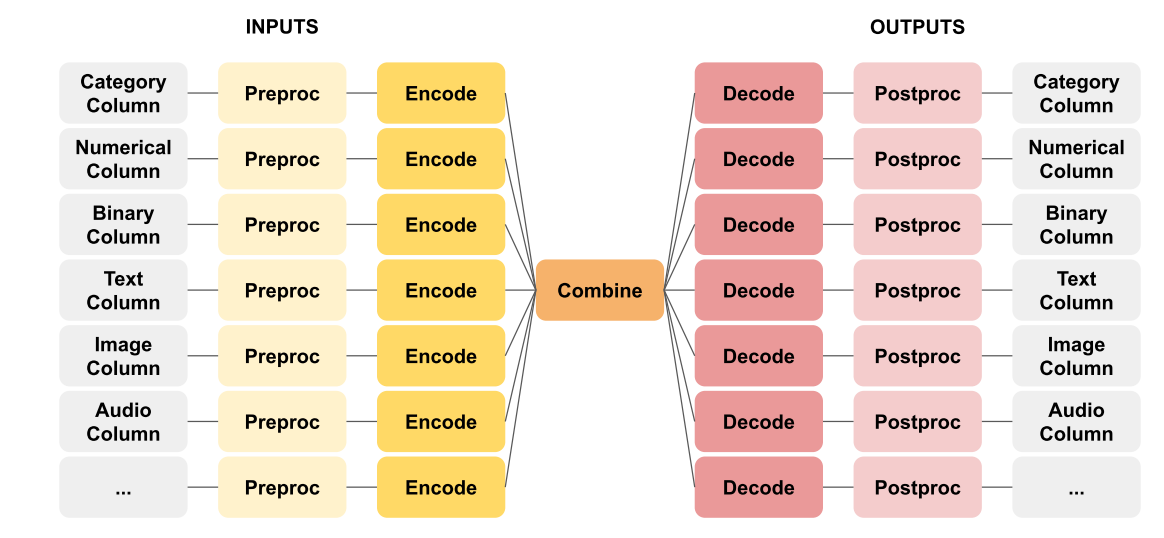
\includegraphics[width=\linewidth,keepaspectratio]{ludwig4}
		\end{center}

\end{frame}


%%%%%%%%%%%%%%%%%%%%%%%%%%%%%%%%%%%%%%%%%%%%%%%%%%%%%%%%%%%
\begin{frame}[fragile]\frametitle{Ludwig Applications}

		\begin{center}
		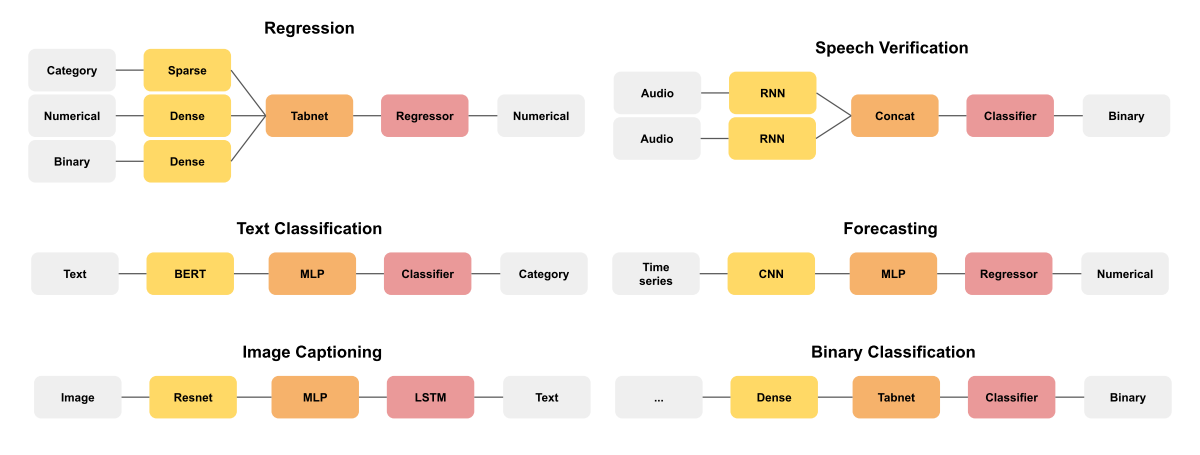
\includegraphics[width=\linewidth,keepaspectratio]{ludwig5}
		\end{center}

\begin{lstlisting}
{Input: [Category|Numerical|Binary], Output: [Numerical}} is a Regression problem 

{Input: [Text], Output: [Category}} is a Text Classification problem
\end{lstlisting}

\end{frame}

%%%%%%%%%%%%%%%%%%%%%%%%%%%%%%%%%%%%%%%%%%%%%%%%%%%%%%%%%%%
\begin{frame}[fragile]\frametitle{Prompt Templating}

		\begin{center}
		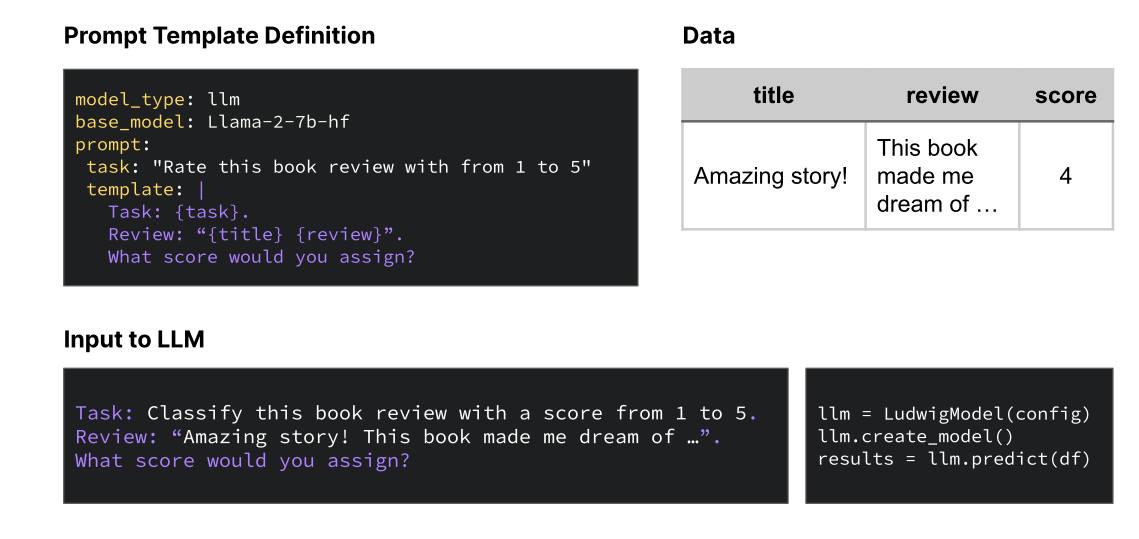
\includegraphics[width=\linewidth,keepaspectratio]{ludwig6}
		\end{center}
		
Ludwig looks at 'Prompt Template Definition' (using column names in `Data') and 'Data' (as 'df') and then internally generates 'Input to LLM' for the row shown

\end{frame}

%%%%%%%%%%%%%%%%%%%%%%%%%%%%%%%%%%%%%%%%%%%%%%%%%%%%%%%%%%%
\begin{frame}[fragile]\frametitle{Declarative-ly Fine-Tune LLMs}

Full-Instruction based fine-tuning for a task. Trains all the layers including embedding, encoding and decoding parts.

		\begin{center}
		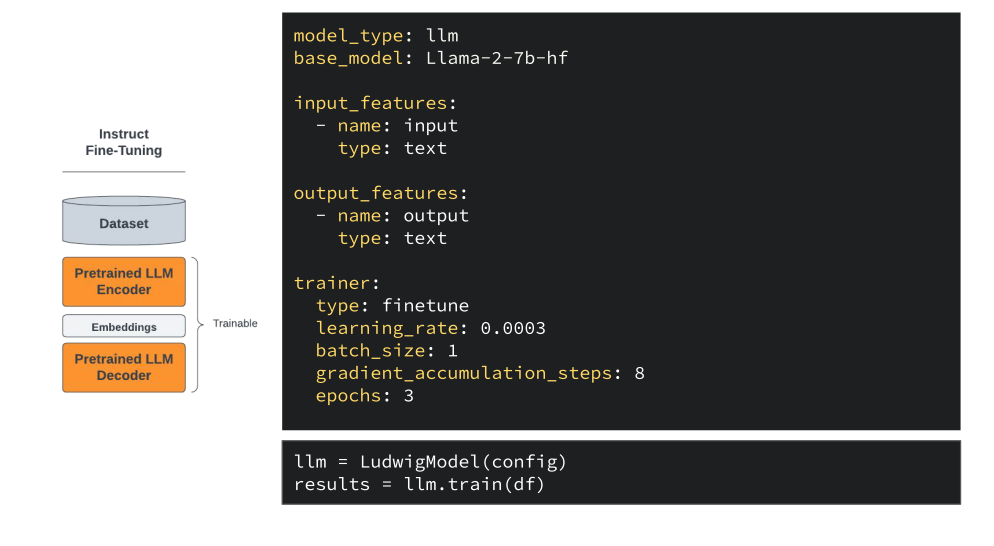
\includegraphics[width=\linewidth,keepaspectratio]{ludwig7}
		\end{center}

\end{frame}

%%%%%%%%%%%%%%%%%%%%%%%%%%%%%%%%%%%%%%%%%%%%%%%%%%%%%%%%%%%
\begin{frame}[fragile]\frametitle{Declaratively Fine-Tune LLMs}

New head 'Classification Decoder' is added for the sentiment analysis task.

		\begin{center}
		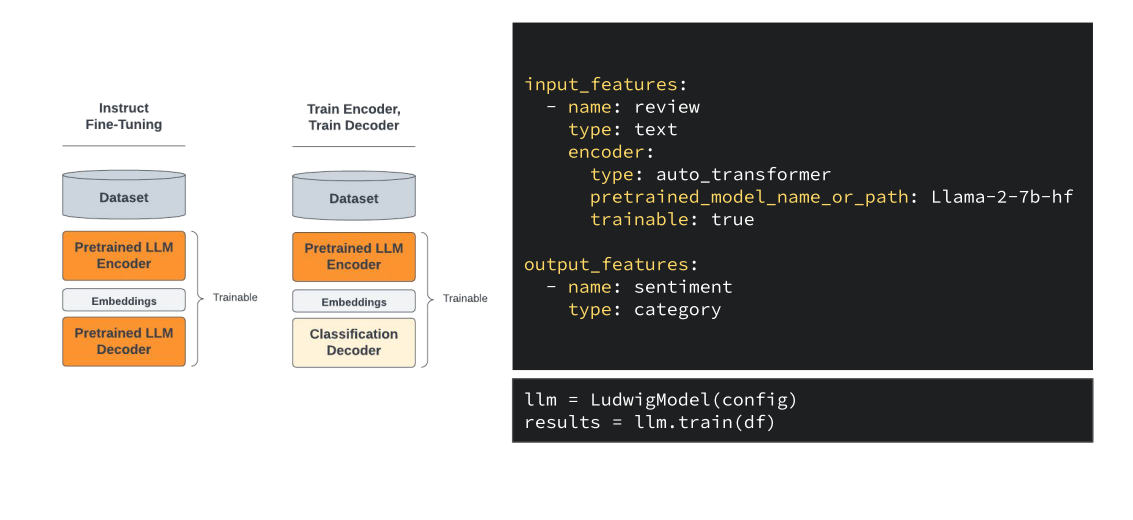
\includegraphics[width=\linewidth,keepaspectratio]{ludwig8}
		\end{center}

\end{frame}

%%%%%%%%%%%%%%%%%%%%%%%%%%%%%%%%%%%%%%%%%%%%%%%%%%%%%%%%%%%
\begin{frame}[fragile]\frametitle{Declaratively Fine-Tune LLMs}

Freezing the Large Language Model.

		\begin{center}
		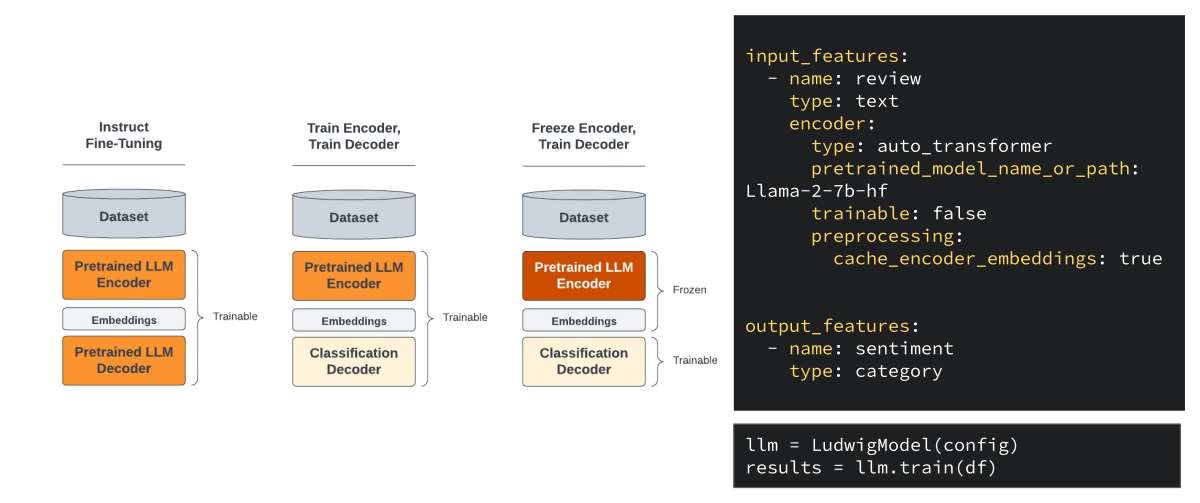
\includegraphics[width=\linewidth,keepaspectratio]{ludwig9}
		\end{center}

\end{frame}

%%%%%%%%%%%%%%%%%%%%%%%%%%%%%%%%%%%%%%%%%%%%%%%%%%%%%%%%%%%
\begin{frame}[fragile]\frametitle{Parameter efficient fine-tuning}

		\begin{center}
		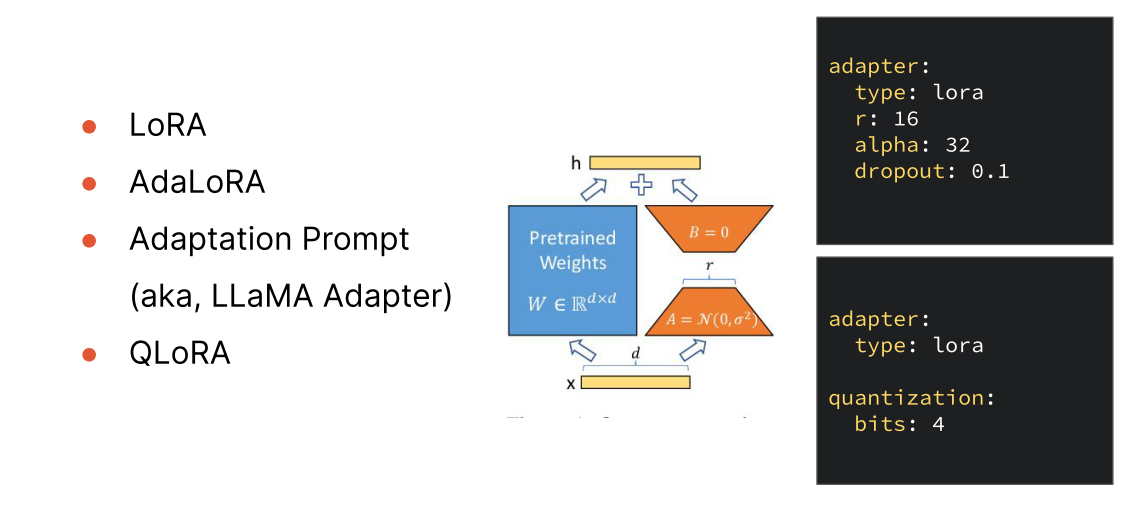
\includegraphics[width=\linewidth,keepaspectratio]{ludwig10}
		\end{center}

\end{frame}

%%%%%%%%%%%%%%%%%%%%%%%%%%%%%%%%%%%%%%%%%%%%%%%%%%%%%%%%%%%
\begin{frame}[fragile]\frametitle{Putting it all together}

		\begin{center}
		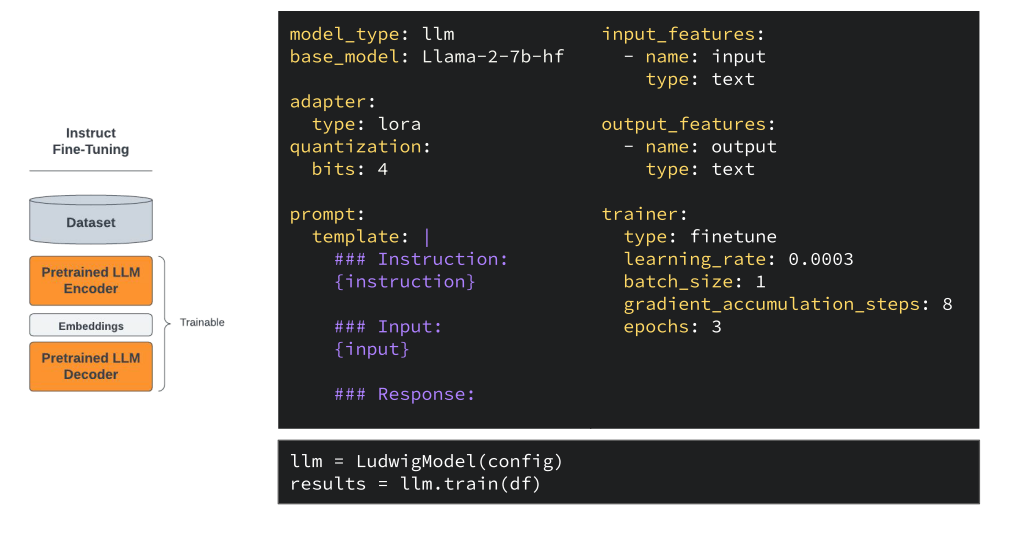
\includegraphics[width=\linewidth,keepaspectratio]{ludwig11}
		\end{center}

\end{frame}

% %%%%%%%%%%%%%%%%%%%%%%%%%%%%%%%%%%%%%%%%%%%%%%%%%%%%%%%%%%%
% \begin{frame}[fragile]\frametitle{Example Application}

% Hands-on Tutorial available at: https://medium.com/google-cloud/gemma-for-gst-4595d5f60b6b
% Or at ``llm\_Gemma\_QnA\_GST\_FAQs\_Ludwig.ipynb''

% \end{frame}

%%%%%%%%%%%%%%%%%%%%%%%%%%%%%%%%%%%%%%%%%%%%%%%%%%%%%%%%%%%%%%%%%%%%%%%%%%%%%%%%%%
\begin{frame}[fragile]\frametitle{Summary}
    \begin{itemize}
        \item Ludwig framework simplifies fine-tuning of LLMs.
        \item Enables efficient adaptation to diverse tasks.
        \item Empowers practitioners to leverage state-of-the-art language models effectively.
    \end{itemize}
\end{frame}
